‌\section{Introducción}
Partiendo del diseño presentado en el trabajo anterior donde se buscó un sistema de venta de telefonía celular que permita tener un alto grado de confiabilidad tanto para el vendedor como para el cliente, que mantenga interconectadas a las distintas partes de la empresa (marketing - ventas - facturación - stock) en todo momento, que automatice algunos procesos internos de la empresa y que agilice y mejore el rendimiento de ventas, se presenta en este trabajo una segunda capa de modelos que pretenden ilustrar la funcionalidad y desenvolvimiento del sistema.\\
\indent Como primer acercamiento a la utilización de la plataforma y su interacción con los distintos actores se incluyen una serie de Diagramas de Actividad en los que se despliegan tanto situaciones de uso abstractas y generales como también representaciones de casos puntuales tal y como se describiera en la sección \textsl{Escenarios} del primer informe. Luego se introduce un Modelo Conceptual con su especificación en $OCL$ con el objeto de \textbf{ME FALTA CHAMUYO ACÁ}. Como tercer acercamiento para entender la confecciòn de este sistema se presentan diversos casos de uso con sus actores, modelo que está íntimamente relacionado con los primeros diagramas de actividad y que expanden el detalle de estas interacciones.\\
\indent Por último, y no por eso menos importante, se incluye un modelo de Máquinas de Estado puesto que resultó oportuna su utilización para graficar de manera más formal cómo se comporta el sistema de ventas a la hora de tener que sincronizar procesos de la misma naturaleza que se realizan en paralelo y para los cuales es fundamental tener concurrencia con el stock de equipos de celular a modo de evitar falsas promesas y situaciones incómodas con los potenciales clientes.\\
\indent Es importante resaltar que a lo largo de este trabajo también se hace foco en la interconexión de estos modelos, característica denominada \textsl{trazabilidad}, la cual es fundamental para lograr comprender de manera integral el problema a través de los distintos acercamientos propuestos.\\

\section{Modelo Conceptual}

\clearpage

\section{Casos de Uso}

\subsection{Casos de Uso MVP}

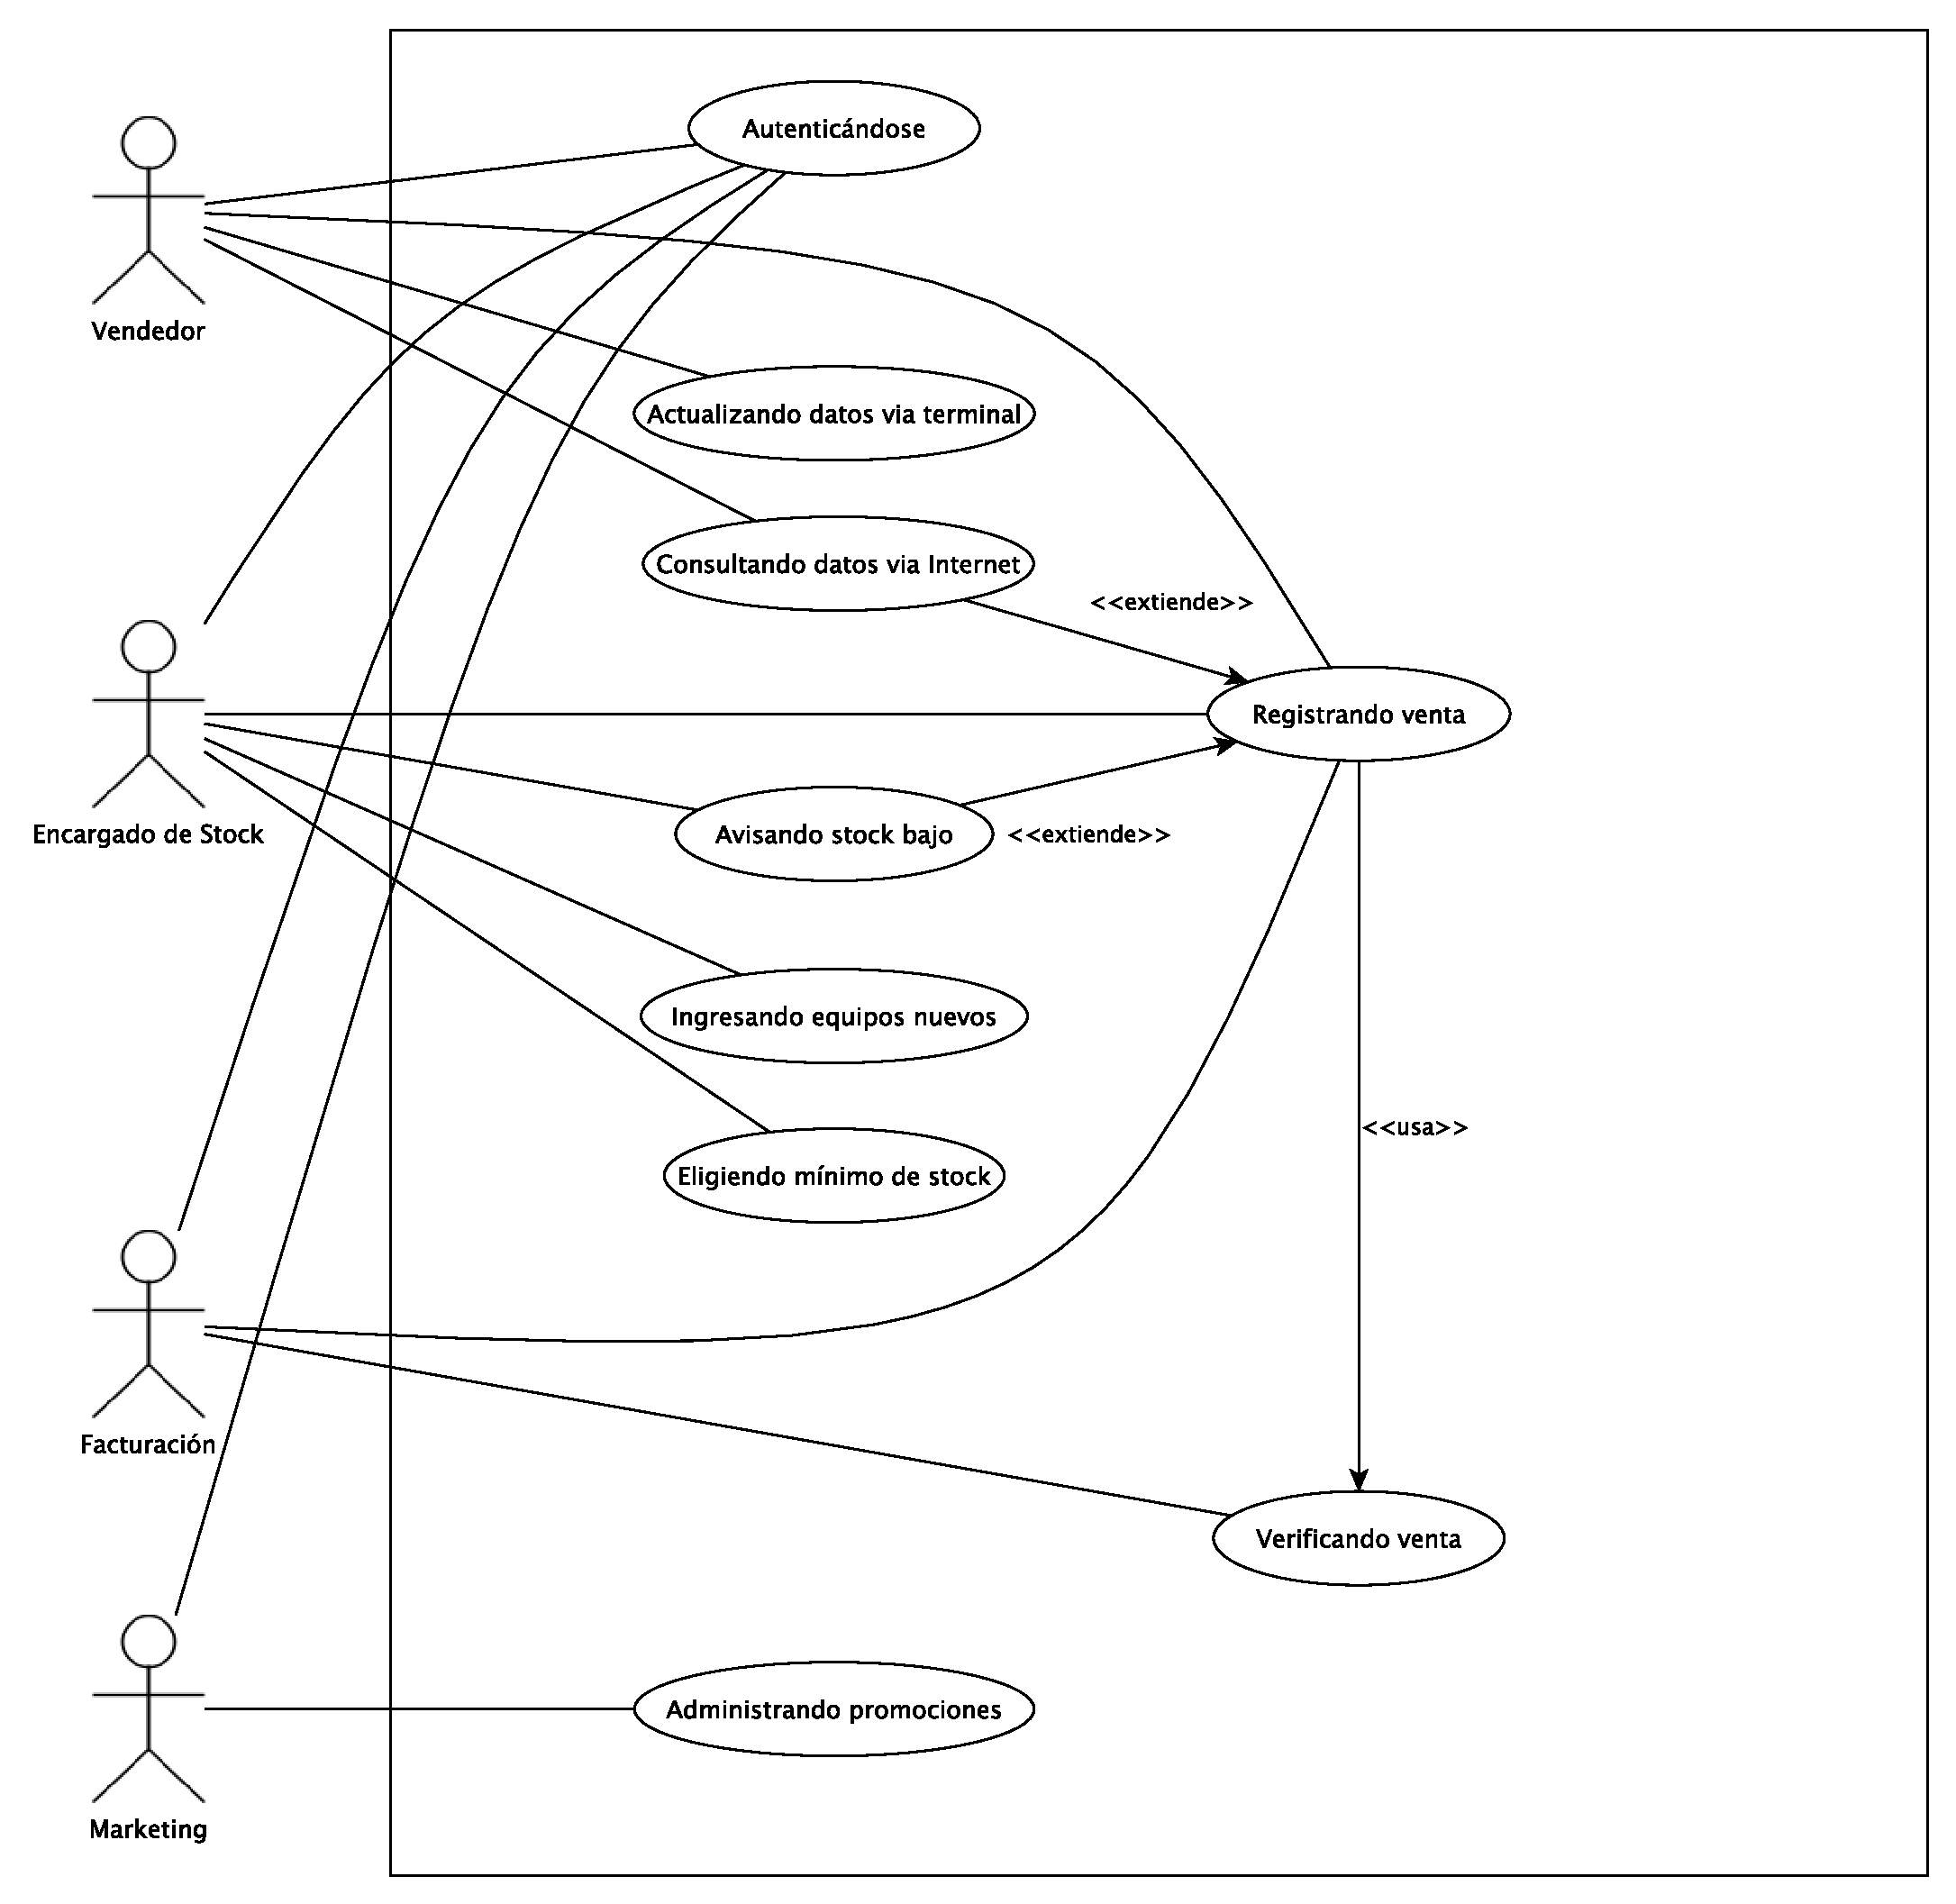
\includegraphics[width=1\textwidth]{./imagenes/casos_de_uso_mvp.pdf}

\subsubsection{Descripción de Casos de Uso}

\begin{tabular}{ | p{7cm} | p{7cm} | }
  \hline
  \multicolumn{2} {|l|} {Caso de Uso: Autenticándose.} \\
  \multicolumn{2} {|l|} {Actores: Vendedor, Encargado de Stock, Facturación, Marketing.} \\
  \multicolumn{2} {|l|} {Post: El usuario está autenticado en el sistema.} \\
  \hline
  Curso Normal & Curso Alternativo\\
  \hline
  1. El usuario ingresa a la interfaz web del sistema. & \\
  2. El usuario ingresa sus credenciales. & \\
  3. El sistema comprueba la validez de las credenciales y las acepta. & 3. El sistema comprueba la validez de las credenciales y las rechaza\\
  4. El usuario queda autenticado en el sistema. & 4. El usuario es redirigido al formulario para reingresar sus credenciales.\\
  \hline
\end{tabular}

\vspace{1cm}

\begin{tabular}{ | p{14cm} | }
  \hline
  Caso de Uso: Actualizando datos via terminal. \\
  Actores: Vendedor. \\
  Pre: El usuario está autenticado en el sistema. \\
  Post: El vendedor tiene actualizados en su dispositivo móvil promociones y datos de clientes. \\
  \hline
  Curso Normal\\
  \hline
  1. El vendedor enchufa su dispositivo móvil en una terminal del sistema ubicada en la oficina. \\
  2. El sistema actualiza automáticamente datos de promociones y clientes. \\
  \hline
\end{tabular}

\vspace{1cm}

\begin{tabular}{ | p{14cm} | }
  \hline
  Caso de Uso: Consultando datos via Internet. \\
  Actores: Vendedor. \\
  Pre: El usuario está autenticado en el sistema. \\
  Post: El vendedor recibe en su dispositivo móvil promociones y datos de clientes. \\
  \hline
  Curso Normal\\
  \hline
  1. El vendedor ingresa nombre del cliente que está visitando en su dispositivo móvil. \\
  2. El sistema busca los datos relacionados al cliente y promociones disponibles para él y los envía al dispositivo móvil del vendedor. \\
  \hline
\end{tabular}

\vspace{1cm}

\begin{tabular}{ | p{14cm} | }
  \hline
  Caso de Uso: Avisando stock bajo. \\
  Actores: Encargado de Stock. \\
  Pre: El usuario está autenticado en el sistema y l stock de alguno de los equipos asociado a promociones vigentes está pronto a agotarse. \\
  Post: El encargado de stock es notificado sobre el equipo pronto a agotarse. \\
  \hline
  Curso Normal\\
  \hline
  1. El sistema marca como reservados los equipos correspondientes con la promoción vendida.\\
  2. El sistema notifica al encargado de stock sobre los equipos reservados.\\
  \hline
\end{tabular}

\vspace{1cm}

\begin{tabular}{ | p{7cm} | p{7cm} | }
  \hline
  \multicolumn{2} {|l|} {Caso de Uso: Verificando venta.} \\
  \multicolumn{2} {|l|} {Actores: Facturación.} \\
  \multicolumn{2} {|l|} {Pre: El usuario está autenticado con el sistema y se registró una venta con stock disponible.} \\
  \multicolumn{2} {|l|} {Post: La venta se confirma y pasa al sistema de facturación.} \\
  \hline
  Curso Normal & Curso Alternativo\\
  \hline
  1. Facturación verifica la situación del cliente y aprueba la venta. & 1. Facturación verifica la situación del cliente y rechaza la venta. \\
  2. Se pasan los datos al sistema de facturación & 2. Se notifica al vendedor que la venta fue rechazada. \\
  \hline
\end{tabular}

\vspace{1cm}

\begin{tabular}{ | p{7cm} | p{7cm} | }
  \hline
   \multicolumn{2} {| p{10cm} |} {Caso de Uso: Registrando venta.} \\
   \multicolumn{2} {| p{10cm} |} {Actores: Vendedor, Encargado de Stock, Facturación.} \\
   \multicolumn{2} {| p{10cm} |} {Pre: El usuario está autenticado con el sistema y el vendedor tiene datos de clientes y promociones actualizados.} \\
   \multicolumn{2} {| p{10cm} |} {Post: Se registra una venta en el sistema.} \\
  \hline
  Curso Normal & Curso Alternativo\\
  \hline
  1. Se extiende con Consultando datos via Internet. & \\
  2. El vendedor decide junto al cliente qué promoción adquirir. & \\
  3. El vendedor ingresa elige en su dispositivo móvil la promoción que su cliente desea. & \\
  4. El sistema verifica que haya suficientes equipos en stock para satisfacer la promoción. & 4. El sistema verifica que los equipos en stock no alcanzan para satisfacer la promoción\\
  5. El sistema marca como reservados los equipos correspondientes con la promoción vendida. & 5. Se notifica al vendedor que la promoción no puede ser vendida. \\
  6. El sistema notifica al encargado de stock sobre los equipos reservados. & \\ 
  7. Se extiende con Avisando stock bajo. & \\
  8. Usa Verificando venta. & \\
  \hline
\end{tabular}

\vspace{1cm}

\begin{tabular}{ | p{14cm} | }
  \hline
  Caso de Uso: Ingresando equipos nuevos. \\
  Actores: Encargado de Stock. \\
  Pre: El usuario está autenticado con el sistema y nuevos equipos fueron ingresados al almacén. \\
  Post: Los nuevos equipos quedan dados de alta en el sistema. \\
  \hline
  Curso Normal\\
  \hline
  1. El usuario actualiza la cantidad de equipos correspondientes a los ingresados recientemente. \\
  \hline
\end{tabular}

\vspace{1cm}

\begin{tabular}{ | p{14cm} | }
  \hline
  Caso de Uso: Administrando promociones. \\
  Actores: Marketing. \\
  Pre: El usuario está autenticado con el sistema. \\
  Post: Se actualizan las promociones disponibles. \\
  \hline
  Curso Normal\\
  \hline
  1. El departamento de Marketing realiza un estudio de mercado para decidir qué promociones ofrecer según tipo de cliente. \\
  2. El usuario ingresado en el sistema crea, edita o borra una promoción. \\
  \hline
\end{tabular}

\subsection{Casos de Uso}

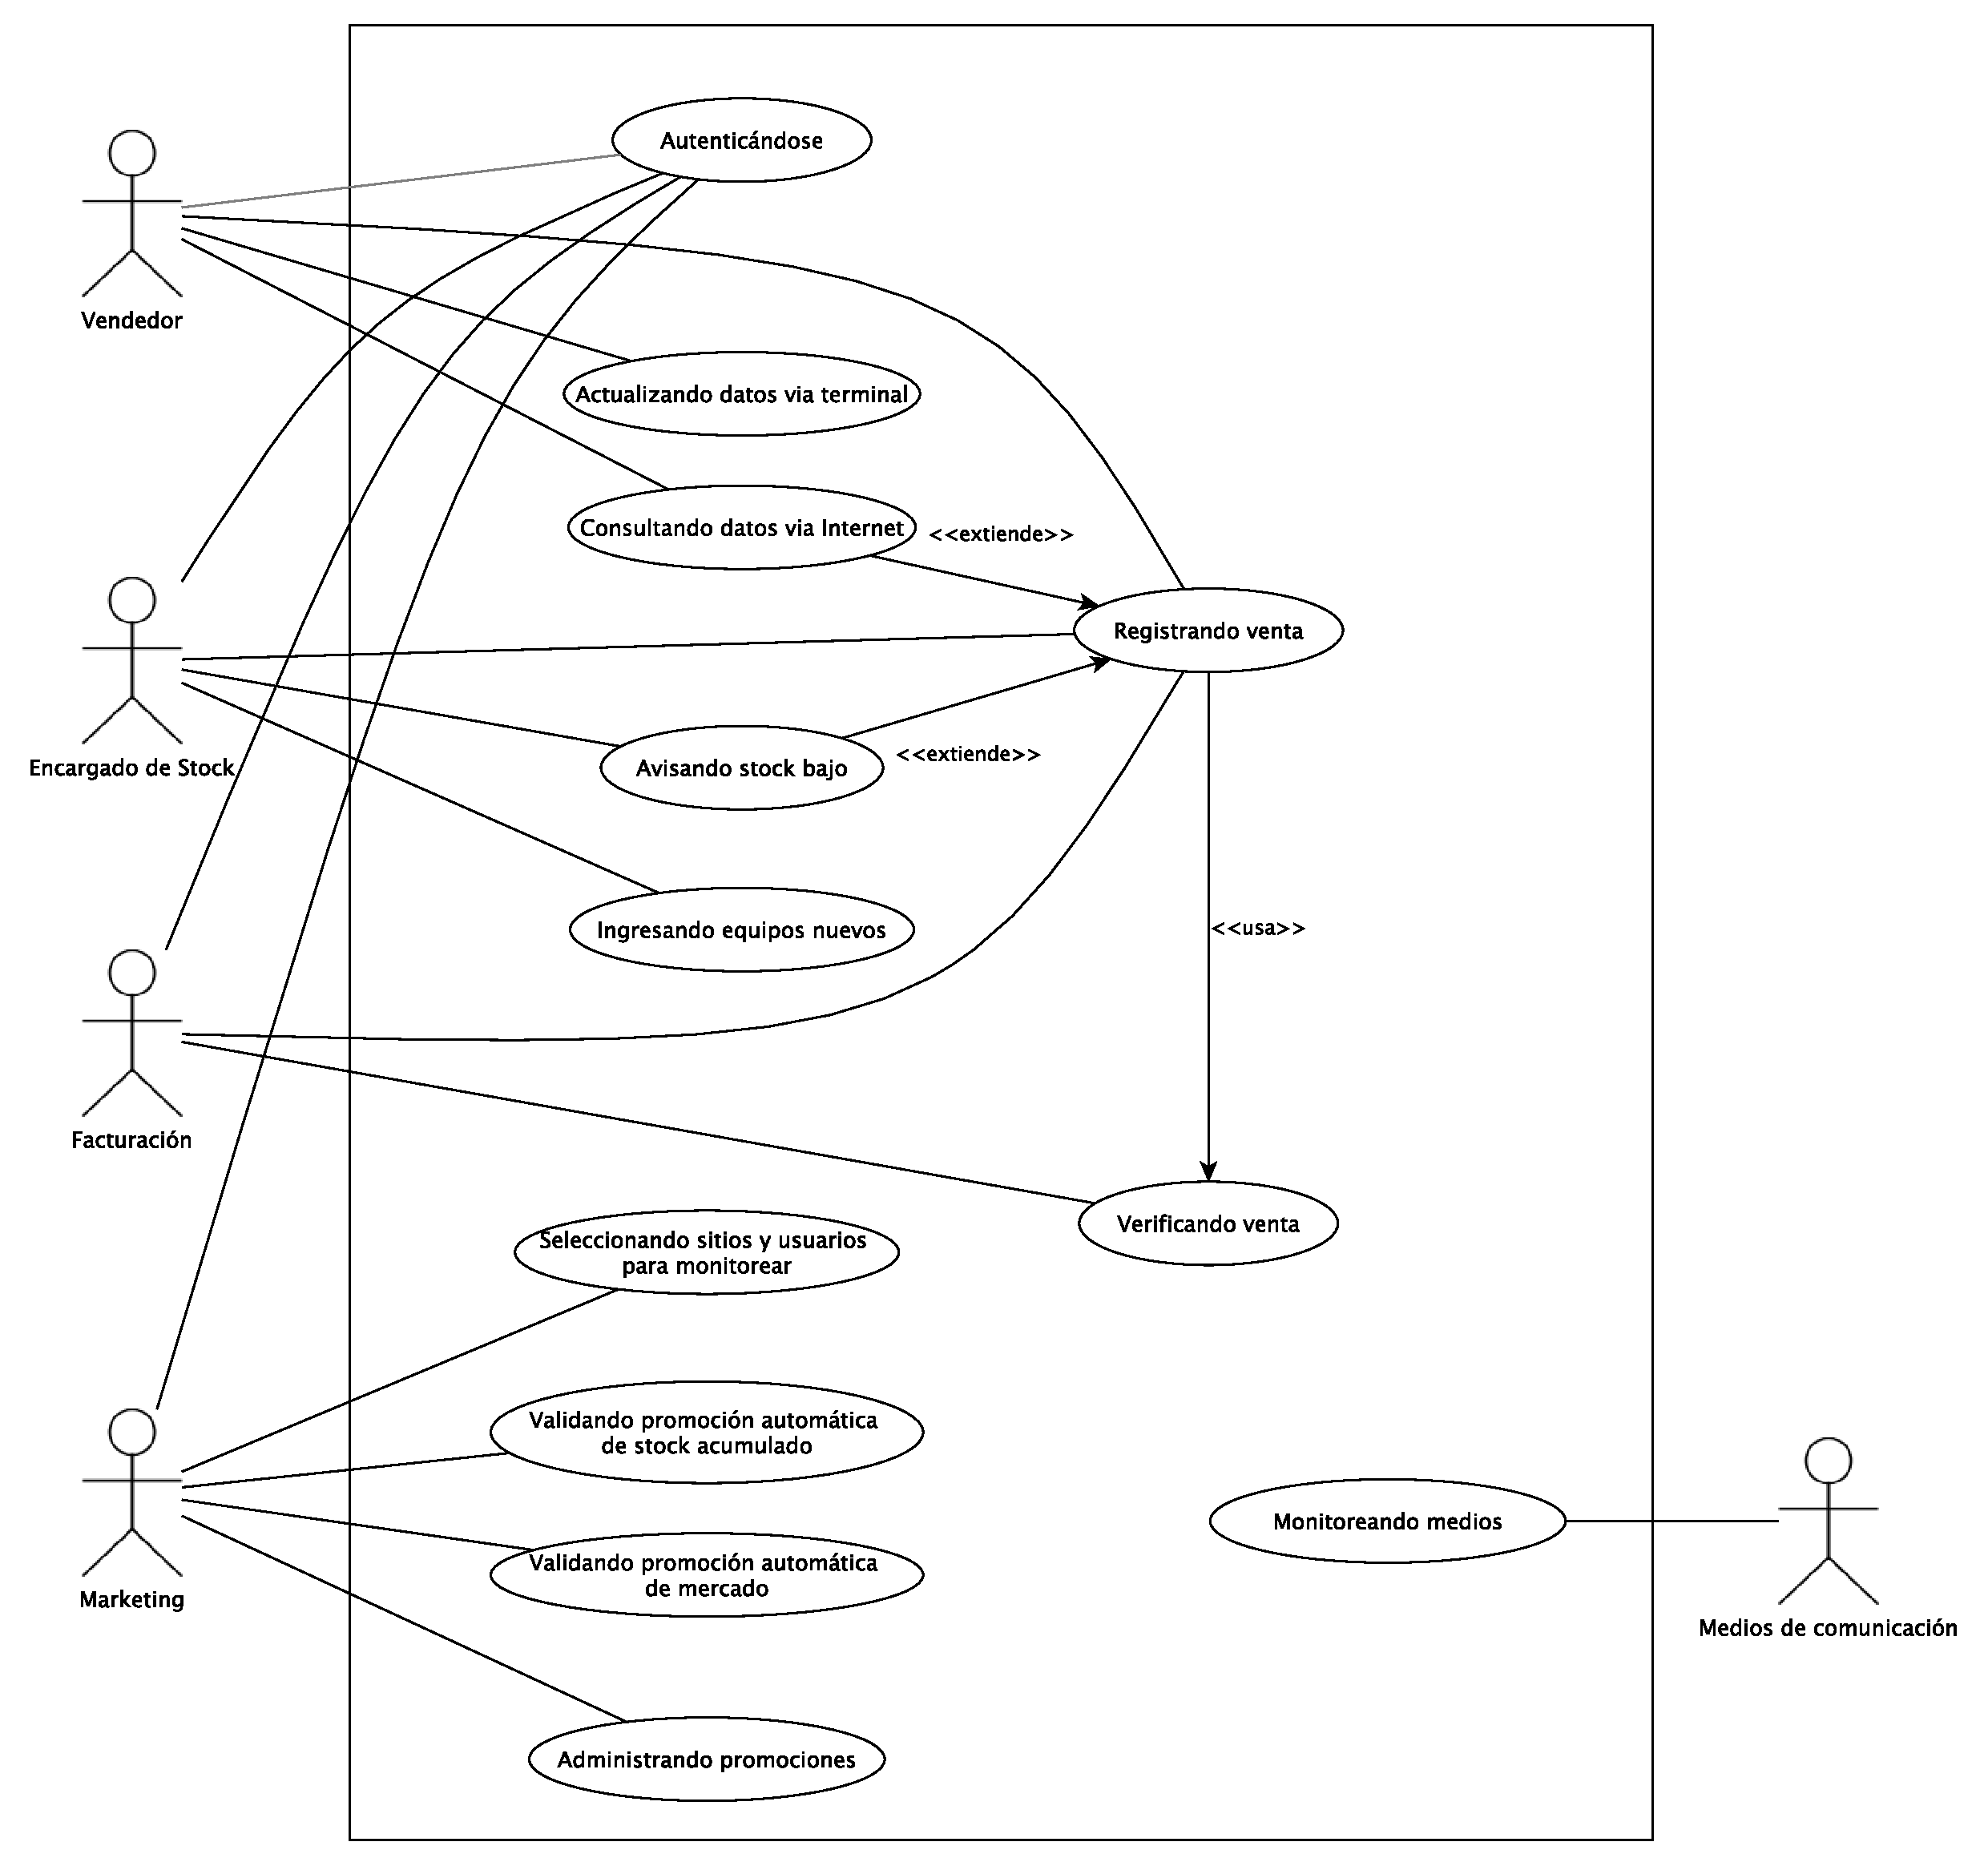
\includegraphics[width=1.3\textwidth, angle=90]{./imagenes/casos_de_uso.pdf}

\clearpage

\subsubsection{Descripción de Casos de Uso}

\begin{tabular}{ | p{7cm} | p{7cm} | }
  \hline
  \multicolumn{2} {|l|} {Caso de Uso: Autenticándose.} \\
  \multicolumn{2} {|l|} {Actores: Vendedor, Encargado de Stock, Facturación, Marketing.} \\
  \multicolumn{2} {|l|} {Post: El usuario está autenticado en el sistema.} \\
  \hline
  Curso Normal & Curso Alternativo\\
  \hline
  1. El usuario ingresa a la interfaz web del sistema. & \\
  2. El usuario ingresa sus credenciales. & \\
  3. El sistema comprueba la validez de las credenciales y las acepta. & 3. El sistema comprueba la validez de las credenciales y las rechaza\\
  4. El usuario queda autenticado en el sistema. & 4. El usuario es redirigido al formulario para reingresar sus credenciales.\\
  \hline
\end{tabular}

\vspace{1cm}

\begin{tabular}{ | p{14cm} | }
  \hline
  Caso de Uso: Actualizando datos via terminal. \\
  Actores: Vendedor. \\
  Pre: El usuario está autenticado en el sistema. \\
  Post: El vendedor tiene actualizados en su dispositivo móvil promociones y datos de clientes. \\
  \hline
  Curso Normal\\
  \hline
  1. El vendedor enchufa su dispositivo móvil en una terminal del sistema ubicada en la oficina. \\
  2. El sistema actualiza automáticamente datos de promociones y clientes. \\
  \hline
\end{tabular}

\vspace{1cm}

\begin{tabular}{ | p{14cm} | }
  \hline
  Caso de Uso: Consultando datos via Internet. \\
  Actores: Vendedor. \\
  Pre: El usuario está autenticado en el sistema. \\
  Post: El vendedor recibe en su dispositivo móvil promociones y datos de clientes. \\
  \hline
  Curso Normal\\
  \hline
  1. El vendedor ingresa nombre del cliente que está visitando en su dispositivo móvil. \\
  2. El sistema busca los datos relacionados al cliente y promociones disponibles para él y los envía al dispositivo móvil del vendedor. \\
  \hline
\end{tabular}

\vspace{1cm}

\begin{tabular}{ | p{14cm} | }
  \hline
  Caso de Uso: Avisando stock bajo. \\
  Actores: Encargado de Stock. \\
  Pre: El usuario está autenticado en el sistema y l stock de alguno de los equipos asociado a promociones vigentes está pronto a agotarse. \\
  Post: El encargado de stock es notificado sobre el equipo pronto a agotarse. \\
  \hline
  Curso Normal\\
  \hline
  1. El sistema marca como reservados los equipos correspondientes con la promoción vendida.\\
  2. El sistema notifica al encargado de stock sobre los equipos reservados.\\
  \hline
\end{tabular}

\vspace{1cm}

\begin{tabular}{ | p{7cm} | p{7cm} | }
  \hline
  \multicolumn{2} {|l|} {Caso de Uso: Verificando venta.} \\
  \multicolumn{2} {|l|} {Actores: Facturación.} \\
  \multicolumn{2} {|l|} {Pre: El usuario está autenticado con el sistema y se registró una venta con stock disponible.} \\
  \multicolumn{2} {|l|} {Post: La venta se confirma y pasa al sistema de facturación.} \\
  \hline
  Curso Normal & Curso Alternativo\\
  \hline
  1. Facturación verifica la situación del cliente y aprueba la venta. & 1. Facturación verifica la situación del cliente y rechaza la venta. \\
  2. Se pasan los datos al sistema de facturación & 2. Se notifica al vendedor que la venta fue rechazada. \\
  \hline
\end{tabular}

\vspace{1cm}

\begin{tabular}{ | p{7cm} | p{7cm} | }
  \hline
   \multicolumn{2} {| p{10cm} |} {Caso de Uso: Registrando venta.} \\
   \multicolumn{2} {| p{10cm} |} {Actores: Vendedor, Encargado de Stock, Facturación.} \\
   \multicolumn{2} {| p{10cm} |} {Pre: El usuario está autenticado con el sistema y el vendedor tiene datos de clientes y promociones actualizados.} \\
   \multicolumn{2} {| p{10cm} |} {Post: Se registra una venta en el sistema.} \\
  \hline
  Curso Normal & Curso Alternativo\\
  \hline
  1. Se extiende con Consultando datos via Internet. & \\
  2. El vendedor decide junto al cliente qué promoción adquirir. & \\
  3. El vendedor ingresa elige en su dispositivo móvil la promoción que su cliente desea. & \\
  4. El sistema verifica que haya suficientes equipos en stock para satisfacer la promoción. & 4. El sistema verifica que los equipos en stock no alcanzan para satisfacer la promoción\\
  5. El sistema marca como reservados los equipos correspondientes con la promoción vendida. & 5. Se notifica al vendedor que la promoción no puede ser vendida. \\
  6. El sistema notifica al encargado de stock sobre los equipos reservados. & \\ 
  7. Se extiende con Avisando stock bajo. & \\
  8. Usa Verificando venta. & \\
  \hline
\end{tabular}

\vspace{1cm}

\begin{tabular}{ | p{14cm} | }
  \hline
  Caso de Uso: Ingresando equipos nuevos. \\
  Actores: Encargado de Stock. \\
  Pre: El usuario está autenticado con el sistema y nuevos equipos fueron ingresados al almacén. \\
  Post: Los nuevos equipos quedan dados de alta en el sistema. \\
  \hline
  Curso Normal\\
  \hline
  1. El usuario actualiza la cantidad de equipos correspondientes a los ingresados recientemente. \\
  \hline
\end{tabular}

\vspace{1cm}

\begin{tabular}{ | p{14cm} | }
  \hline
  Caso de Uso: Administrando promociones. \\
  Actores: Marketing. \\
  Pre: El usuario está autenticado con el sistema. \\
  Post: Se actualizan las promociones disponibles. \\
  \hline
  Curso Normal\\
  \hline
  1. El departamento de Marketing realiza un estudio de mercado para decidir qué promociones ofrecer según tipo de cliente. \\
  2. El usuario ingresado en el sistema crea, edita o borra una promoción. \\
  \hline
\end{tabular}

\vspace{1cm}

\begin{tabular}{ | p{14cm} | }
  \hline
  Caso de Uso: Seleccionando sitios y usuarios para monitorear. \\
  Actores: Marketing. \\
  Pre: El usuario está autenticado con el sistema. \\
  Post: El sistema puede comenzar a monitorear medios. \\
  \hline
  Curso Normal\\
  \hline
  1. El usuario selecciona qué usuarios de redes sociales y sitios corporativos el sistema deberá monitorear. \\
  \hline
\end{tabular}

\vspace{1cm}

\begin{tabular}{ | p{14cm} | }
  \hline
  Caso de Uso: Validando promoción automática de stock acumulado. \\
  Actores: Marketing. \\
  Pre: El usuario está autenticado con el sistema. \\
  Post: Se crea una promoción en base al stock acumulado, autorizada por Marketing. \\
  \hline
  Curso Normal\\
  \hline
  1. El sistema detecta que se acumuló mucho stock de un determinado equipo. \\
  2. El sistema crea una promoción basada en el stock acumulado de dicho equipo y notifica al usuario. \\
  3. El usuario ve la promoción y la valida. \\
  4. La promoción pasa a estar disponible para los vendedores. \\
  \hline
\end{tabular}

\vspace{1cm}

\begin{tabular}{ | p{14cm} | }
  \hline
  Caso de Uso: Validando promoción automática de mercado. \\
  Actores: Marketing. \\
  Pre: El usuario está autenticado con el sistema. \\
  Post: Se crea una promoción en base al estado del mercado, autorizada por Marketing. \\
  \hline
  Curso Normal\\
  \hline
  1. El usuario ve la promoción y la valida. \\
  2. La promoción pasa a estar disponible para los vendedores. \\
  \hline
\end{tabular}

\vspace{1cm}

\begin{tabular}{ | p{14cm} | }
  \hline
  Caso de Uso: Monitoreando medios.\\
  Actores: Medios de Comunicación. \\
  Pre: Se seleccionaron sitios y usuarios para monitorear. \\
  Post: El sistema realizó el monitoreo de los medios de comunicación en Internet según las preferencias seleccionadas. \\
  \hline
  Curso Normal\\
  \hline
  1. El sistema monitorea los medios de comunicación por internet asociados a los usuarios de redes sociales y sitios de la competencia. \\
  \hline
\end{tabular}

\vspace{1cm}

\begin{tabular}{ | p{14cm} | }
  \hline
  Caso de Uso: Recibiendo informe de monitoreo. \\
  Actores: Marketing. \\
  Pre: El usuario está autenticado con el sistema y se el sistema monitoreó los medios de comunicación. \\
  Post: El usuario recibe un informe producto del monitoreo del mercado pudiendo crear una promoción acorde a él. \\
  \hline
  Curso Normal\\
  \hline
  1. El sistema envía un informe con los detalles del estado del mercado al usuario. \\
  2. El usuario crea la promoción sugerida por el informe. \\
  3. Se extiende con Validando promoción automática de mercado. \\
  \hline
\end{tabular}

\clearpage

\section{Diagramas de actividad}

\clearpage
